% Preview body

\subsection{Presentation}

\paragraph{Home} (Figure~\ref{fig:HiHome})

\marginpar{%
	\begin{overpic}[width=\marginparwidth]
		{img/secondPrototype/home}
	\end{overpic}
	\captionof{figure}{The Home screen}\label{fig:HiHome}
}

The user is at first presented with three main options to choose from.
\begin{enumerate}
	\item Make a new booking; this button takes the user to a page to input
		their search criteria. (Figure~\ref{fig:HiSearch})
	\item View their bookings; this button allows the user to see past and
		present bookings. (Figure~\ref{fig:HiBookings})
	\item Input their details; this page allows the user to specify a number
		of details about themselves:

		\begin{enumerate}
			\item Their concession status so they potential offers and
				discounts can be highlighted in the search results.
			\item Default search preferences if they regularly search for the
				same sport, location or time when looking to make a booking.
		\end{enumerate}
	\item The home button is repeated on every page and provides the user with
		a quick way to return to this home screen.
\end{enumerate}

\paragraph{My Bookings} (Figure~\ref{fig:HiBookings})

\marginpar{%
	\begin{overpic}[width=\marginparwidth]
		{img/secondPrototype/bookings}
	\end{overpic}
	\captionof{figure}{Current and past bookings screen}\label{fig:HiBookings}
}

This page shows scrollable lists of current and past bookings the user has
made. This allows the user to find details about past bookings if they want to
repeat a search or contact the location. The user may also be able to cancel a
current booking if the particular location they have booked allows them to.

\paragraph{Individual Current Booking Page} (Figure~\ref{fig:HiIndBooking})

\marginpar{%
	\begin{overpic}[width=\marginparwidth]
		{img/secondPrototype/indiv_booking}
	\end{overpic}
	\captionof{figure}{Current booking details screen}\label{fig:HiIndBooking}
}

This page displays information for a current booking.
\begin{enumerate}
	\item A share button; this will display the phone's default share options.
		Typically this will allow the user to share information about the
		booking through other applications on the phone such as email or other
		messaging services.
	\item If the location of this booking allows customers to change booking
		times, this will bring up a search results page, similar to
		figure~\ref{fig:HiList}, showing available booking slots at similar
		times at this location.
	\item The details tab has buttons to call the location, visit their
		website, get directions to the location and also highlights if the
		location has parking facilities. In addition to this, the weather
		prediction for this location at the time of the booking is displayed.
	\item An button to cancel the booking; a prompt will be displayed asking
		the user to confirm that they definitely wish to cancel the booking.
		If the location does not allow booking cancellations, this button will
		be greyed out and attempts to press the button will result in a message
		explaining the reason a cancellation cannot be made.
\end{enumerate}

\paragraph{Search} (Figure~\ref{fig:HiSearch})

\marginpar{%
	\begin{overpic}[width=\marginparwidth]
		{img/secondPrototype/search}
	\end{overpic}
	\captionof{figure}{The main search screen}\label{fig:HiSearch}
}

This is the main search screen which displays the current criteria in the
search and allows the user to change this criteria viewing the results that
match this criteria. The user can choose to search after defining any number of
the four criteria.
\begin{enumerate}
	\item Help button; displays hovering annotations describing what each part
		of the page is for.
	\item Reset search button; this resets the search criteria to the default
		settings chosen on the My Details page. If the user has not entered
		these details before then the sport selection will be default to all,
		location to 5km within the user's current location, date to today and
		time to all.
	\item Past booking button; this brings up a drop down list of previous
		bookings. If one of these bookings is chosen, all the search criteria
		will change to match that booking apart from the date which will remain
		unchanged.
	\item Sport selection button with icons that show what is currently
		selected.  Pressing this leads to figure~\ref{fig:HiSport}.
	\item Location button leading to figure~\ref{fig:HiLocation}.
	\item Date button leading to figure~\ref{fig:HiDate}.
	\item Time button leading to figure~\ref{fig:HiTime}.
	\item Search button leading to figure~\ref{fig:HiList} to display results
		matching the current search criteria.
	\item A basket icon which leads to the basket page which displays all
		booking slots a user currently has added to their basket but have yet
		to confirm and pay for.
\end{enumerate}

\paragraph{Sport Selection} (Figure~\ref{fig:HiSport})

\marginpar{%
	\begin{overpic}[width=\marginparwidth]
		{img/secondPrototype/sport}
	\end{overpic}
	\captionof{figure}{The sport selection screen}\label{fig:HiSport}
}

The user can choose to search for as many sports at once as they wish.
\begin{enumerate}
	\item Drop down to choose to display different groups of sport such as
		outdoor sports, indoor sports, teams sports and favourites which are
		defined on the My Details page.
	\item Select all button; this will check all sports currently displayed on
		the page. If all sports are selected, this button changes to clear all
		instead.
	\item Each sport toggles between selected and unselected when pressed.
	\item Done button; this returns the user to the search page. This the same
		for all specific search criteria pages. (Figure~\ref{fig:HiSearch})
	\item Help button; displays hovering annotations describing what each part
		of the page is for.
\end{enumerate}

\paragraph{Location Selection} (Figure~\ref{fig:HiLocation})

\marginpar{%
	\begin{overpic}[width=\marginparwidth]
		{img/secondPrototype/location}
	\end{overpic}
	\captionof{figure}{The location selection screen}\label{fig:HiLocation}
}

The user can choose to to search within a distance from their current
location or specify a particular location via its postcode or area
name.
\begin{enumerate}
	\item Find location; a button which sets the location using the user's
		current location.
	\item Location input text field; when the chooses the first button, this
		is automatically changed to the postcode of their current location.
		The user can also type in this field. As they are typing, suggestions
		will appear in a drop down box to help speed up their search.
	\item A slider bar to determine how far from the chosen location the user
		would like to search.
	\item Public transport; if the checkbox is ticked, the user can choose
		to search for locations which are within a specified journey time
		on public transport such as local buses and trains.
	\item Checkboxes for including in the search only those locations which
		have disabled access and parking facilities.
	\item Help button; displays hovering annotations describing what each part
		of the page is for.
\end{enumerate}

\paragraph{Date Selection} (Figure~\ref{fig:HiDate})

\marginpar{%
	\begin{overpic}[width=\marginparwidth]
		{img/secondPrototype/date}
	\end{overpic}
	\captionof{figure}{The date selection screen}\label{fig:HiDate}
}

All dates which are higlighted on this page will be included in the
search.
\begin{enumerate}
	\item Select all; highlights all dates in the shown month. This button
		changes to clear all when all dates are already selected.
	\item Day headings; when a day is pressed, all the dates on the page for
		that day are highlighted.
	\item The user can either touch a date to highlight it or swipe across multiple
		dates to highlight many dates in one go.
	\item Help button; displays hovering annotations describing what each part
		of the page is for including instructions on using swiping gestures
		to select multiple dates.
\end{enumerate}

\paragraph{Time Selection} (Figure~\ref{fig:HiTime})

\marginpar{%
	\begin{overpic}[width=\marginparwidth]
		{img/secondPrototype/time}
	\end{overpic}
	\captionof{figure}{The time selection screen}\label{fig:HiTime}
}

All hours which are highlighted on this page will be included in the
search.
\begin{enumerate}
	\item AM and PM buttons; when the am is pressed all morning hours are toggled
		on or off, likewise for pm.
	\item The user can either touch an hour to highlight it or swipe across
		multiple times times highlight many times at once.
	\item Help button; displays hovering annotations describing what each part
		of the page is for including instructions on using swiping gestures
		to select multiple times.
\end{enumerate}

\paragraph{List Results} (Figure~\ref{fig:HiList})

\marginpar{%
	\begin{overpic}[width=\marginparwidth]
		{img/secondPrototype/list}
	\end{overpic}
	\captionof{figure}{The map results screen}\label{fig:HiList}
}

This is the default view for search results. Results can be sorted
by distance, time or price and grouped by sport or location. The user
can change the default sort and grouping options on their my details
page.
\begin{enumerate}
	\item Button to return to the search page and amend the search criteria.
	\item Toggle buttons to change how the results are sorted.
	\item Toggle buttons to change how the results are grouped. By default,
		the results are not grouped. An example is shown in figure~\ref{fig:HiListGroup}
		of results grouped by sport. When grouped, a user can expand a chosen
		sport to see all results for that particular sport. These items will
		be also be sorted by the chosen sort option.
	\item Scrollable list of results. The user is shown an icon for the sport,
		the name of the location, the time and date of the booking, the price
		and the distance of the location from their chosen search location.
		Selecting a particular booking slot takes the user to the page in
		figure~\ref{fig:HiIndResult}.
	\item Toggle bar for switching between list and map search view. (Figure~\ref{fig:HiMap})
\end{enumerate}
\marginpar{%
	\begin{overpic}[width=\marginparwidth]
		{img/secondPrototype/list_group}
	\end{overpic}
	\captionof{figure}{The map results screen}\label{fig:HiListGroup}
}

\begin{figure}[htbp]
	\centering
	\begin{subfigure}[b]{0.45\textwidth}
		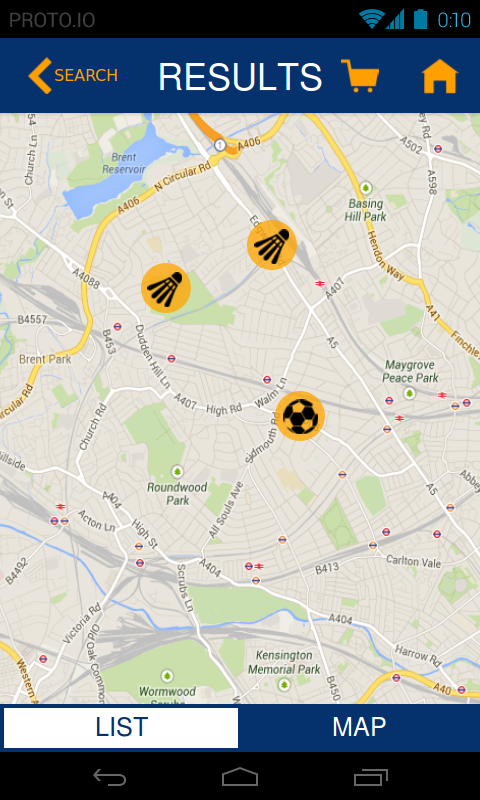
\includegraphics[width=\textwidth]{img/secondPrototype/map}
		\caption{The map results screen}\label{fig:HiMap}
	\end{subfigure}%
	\qquad
	\begin{subfigure}[b]{0.45\textwidth}
		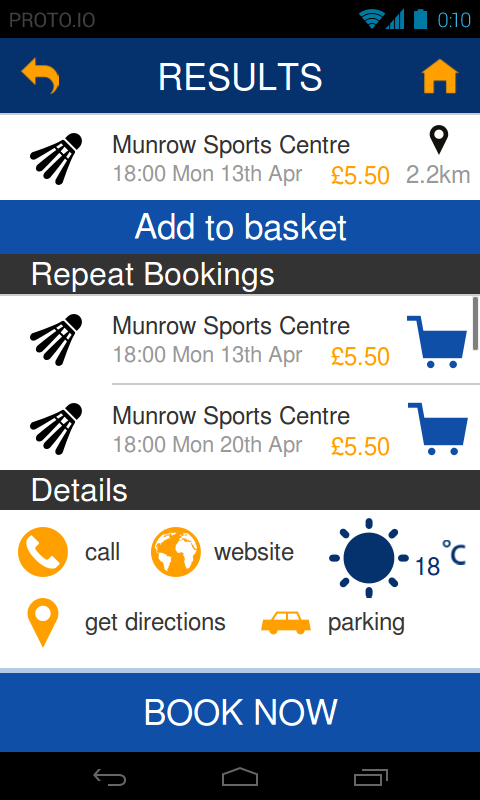
\includegraphics[width=\textwidth]{img/secondPrototype/indiv_result}
		\caption{Screen for a booking slot}\label{fig:HiIndResult}
	\end{subfigure}
	\caption{}\label{fig:MapResult}
\end{figure}

\paragraph{Map Results}

(Figure~\ref{fig:HiMap})

%\marginpar{%
%	\begin{overpic}[width=\marginparwidth]
%		{img/secondPrototype/map}
%	\end{overpic}
%	\captionof{figure}{The map results screen}\label{fig:HiMap}
%}

Results can also be viewed on a map which is navigable in the same
way as the phone's native map application.
\begin{enumerate}
	\item Icons on the map represent a specific venue. If only one sport is
		available at that venue then the picture icon will represent that
		sport. If more than one sport is available, then there will be a plus
		sign to show that multiple sports are available. When pressed, a
		scrollable list is displayed on the screen similar to that in
		figure~\ref{fig:HiListGroup}.
	\item Toggle bar to navigate back to the list view in
		figure~\ref{fig:HiList}.
\end{enumerate}

\paragraph{Individual Result}

(Figure~\ref{fig:HiIndResult})

%\marginpar{%
%	\begin{overpic}[width=\marginparwidth]
%		{img/secondPrototype/indiv_result}
%	\end{overpic}
%	\captionof{figure}{Screen for a booking slot}\label{fig:HiIndResult}
%}
\begin{enumerate}
	\item Button to add the displayed booking to the user's basket so they can
		continue searching before paying.
	\item Scrollable list of bookings for the same sport and location at the
		same time in future weeks so the user can purchase several weeks at
		once if they know they want to play weekly. The basket icon adds the
		booking to the basket.
	\item Details about the location and a weather prediction for the time of
		the chosen booking.
	\item Book now button; takes the user an external pay application to pay
		for booking before returning them to this page. The book now button
		will then change to a link to the page for this current booking as
		in figure~\ref{fig:HiIndBooking} so they can make amendments to their
		booking at share details to their friends.
\end{enumerate}
